\begin{multicols}{2}
\section*{Problem setting}
\begin{centering}
{\large \bf Cellular networks are variable.}
\begin{center}
\def\svgwidth{0.75\columnwidth}\input{allcapacity.pdf_tex}
\end{center}
\end{centering}

\begin{centering}
{\large \bf Cellular networks are too reliable.}
\begin{center}
{\bf \huge
\def\svgwidth{0.75\columnwidth}\input{pings.pdf_tex}
}
\end{center}
\end{centering}

{\large \bf Interactive apps perform poorly because they are reactive.}

\section*{Sprout's goal}
{\large \bf
\begin{center}
Maximize throughput subject to a bounded risk of delay exceeding 100 ms.
\end{center}
}

\section*{How it works}
{\large \bf
\begin{itemize}
\item {\textbf Inference:} Infer probability distribution of link speeds from packet arrivals.
\item {\textbf Prediction:} Predict future link speed.
\item {\textbf Control:} Send as much as possible, but ensuring a 95 \% chance that all packets are delivered within 100 ms.
\end{itemize}
}
\begin{centering}
\def\svgwidth{0.85 \columnwidth}\input{sprout-model.pdf_tex}
\end{centering}

\section*{Inference}
\begin{center}
\def\svgwidth{0.7 \columnwidth}\input{vz-inter.pdf_tex}
\end{center}
{\large \bf
At the receiver:
\begin{itemize}
\item Maintain a probability distribution over link rates.
\item Model receiver's arrivals as a Poisson process with a time-varying rate $\lambda$.
\item Observe number of bytes $k$ that arrived in a tick of duration $\tau$.
\item Compute the likelihood $L(x)$ that a Poisson process with rate $\lambda$ generated $k$ bytes.
      \begin{equation}
       L(x) = \frac{(x.\tau)^{k}}{k!}exp(-x.\tau)
      \end{equation}
\item Update current probability distribution using $L(x)$
      \begin{equation}
       F(x) = Pr_{old}(\lambda = x)*L(x)
      \end{equation}
\item Normalize the new probabilities $F(x)$, so that they sum to unity.
\end{itemize}
}

\section*{Prediction}
{\large \bf
At the receiver:
\begin{itemize}
\item Model evolution of link rates as Brownian motion with constant volatility $\sigma$.
\item Explicitly model outages, using outage escape rate $\lambda_{z}$.
\item Cautious forecast: Find the 5th percentile of the cumulative number of packet deliveries for a certain number of ticks in the future.
\item Send back forecast to sender.
\item Almost all steps are precalculated.
\end{itemize}
}


\section*{Control}
{\large \bf
At the sender:
\begin{itemize}
\item Determine the cumulative number of bytes delivered 100 ms into the future.
\item Subtract number of bytes already in queue.
\item Remaining bytes are ``safe" to send.
\end{itemize}
}

\begin{centering}
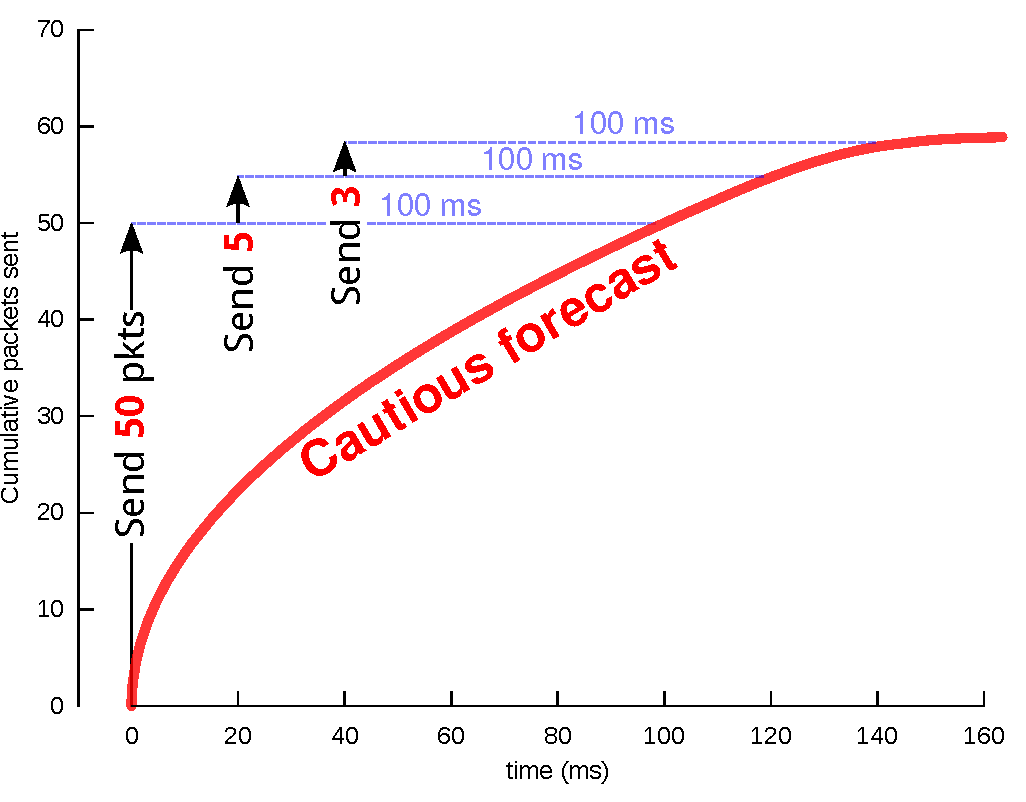
\includegraphics[width=0.5\columnwidth]{forecast-final.pdf}

\end{centering}


\section*{Evaluation}
{\large \bf
\begin{itemize}
\item Saturate a cellular link in both the uplink and downlink directions.
\item Playback trace in a trace-driven link emulator.
\item Measure total throughput and end-to-end delay for reconstructing 95 \% of the signal.
\item Also evaluated Sprout-EWMA, a simplified variant of Sprout:
      \begin{itemize}
      \item At the receiver, estimate link rate using a moving average filter.
      \item Send link rate estimate to the sender, with no forecast.
      \end{itemize}
\item All source code was \textbf{frozen before data collection}.
\end{itemize}
}

{\large \bf
\begin{center}
\textbf{Sprout parameters used in evaluation} \\
\begin{tabular}{|l|l|}
\hline
Volatility $\sigma$: fixed @ & $200~\frac{\textrm{pkts}/s}{\sqrt{s}}$ \\
\hline
Expected outage time $1/\lambda_z$: & $1~s$ \\
\hline
Tick length: & $20~ms$ \\
\hline
Forecast length: & $160~ms$ \\
\hline
Delay target: & $100~ms$ \\
\hline
Risk tolerance: & $5 \%$ \\
\hline
\end{tabular}
\end{center}
}
\vspace{\baselineskip}


%%%\section*{6.829 contest}
%%%\begin{itemize}
%%%\item one
%%%\item two
%%%\item thre
%%%\end{itemize}
%%%
\section*{Results}
\subsection*{Sprout outperforms other end-to-end protocols}
\begin{center}
LTE Networks
\end{center}

\begin{center}
\def\svgwidth{0.44\columnwidth}{\footnotesize  \bf \input{VerizonLTE-Downlink.pdf_tex}}
\hspace{0.1\columnwidth}
\def\svgwidth{0.44\columnwidth}{\footnotesize  \bf \input{ATTLTE-Downlink.pdf_tex}}
\end{center}

\begin{center}
3G Networks
\end{center}

\begin{center}
\def\svgwidth{0.44\columnwidth}{\footnotesize  \bf \input{T-Mobile3GUMTS-Downlink.pdf_tex}}
\hspace{0.1\columnwidth}
\def\svgwidth{0.44\columnwidth}{\footnotesize \bf  \input{Verizon3G1xEV-DO-Downlink.pdf_tex}}
\end{center}

\subsection*{Sprout competes with AQM even though it is end-to-end}
\begin{center}
\def\svgwidth{0.44\columnwidth}\footnotesize \bf \input{Codels.pdf_tex}
\end{center}

\subsection*{Sprout, used as a tunnel, successfully isolates competing traffic}
\begin{center}
{\large \bf
\noindent \begin{tabular}{|l|l|l|l|}
\hline
& Direct & via Sprout & Benefit \\
\hline
\hline
Cubic throughput & 8336 kbps & 3776 kbps & \cellcolor{red!20}$0.5 \times$ (= worse) \\
Skype throughput & 78 kbps & 490 kbps & \cellcolor{blue!20}$6 \times$ \\
Skype 95\% delay & 6.0~s & 0.17~s & \cellcolor{blue!20}$35 \times$ \\
\hline
\end{tabular}
}
\end{center}

\end{multicols}
